\pagestyle{plain}

\cleardoublepage

\newpage
\begin{center}
	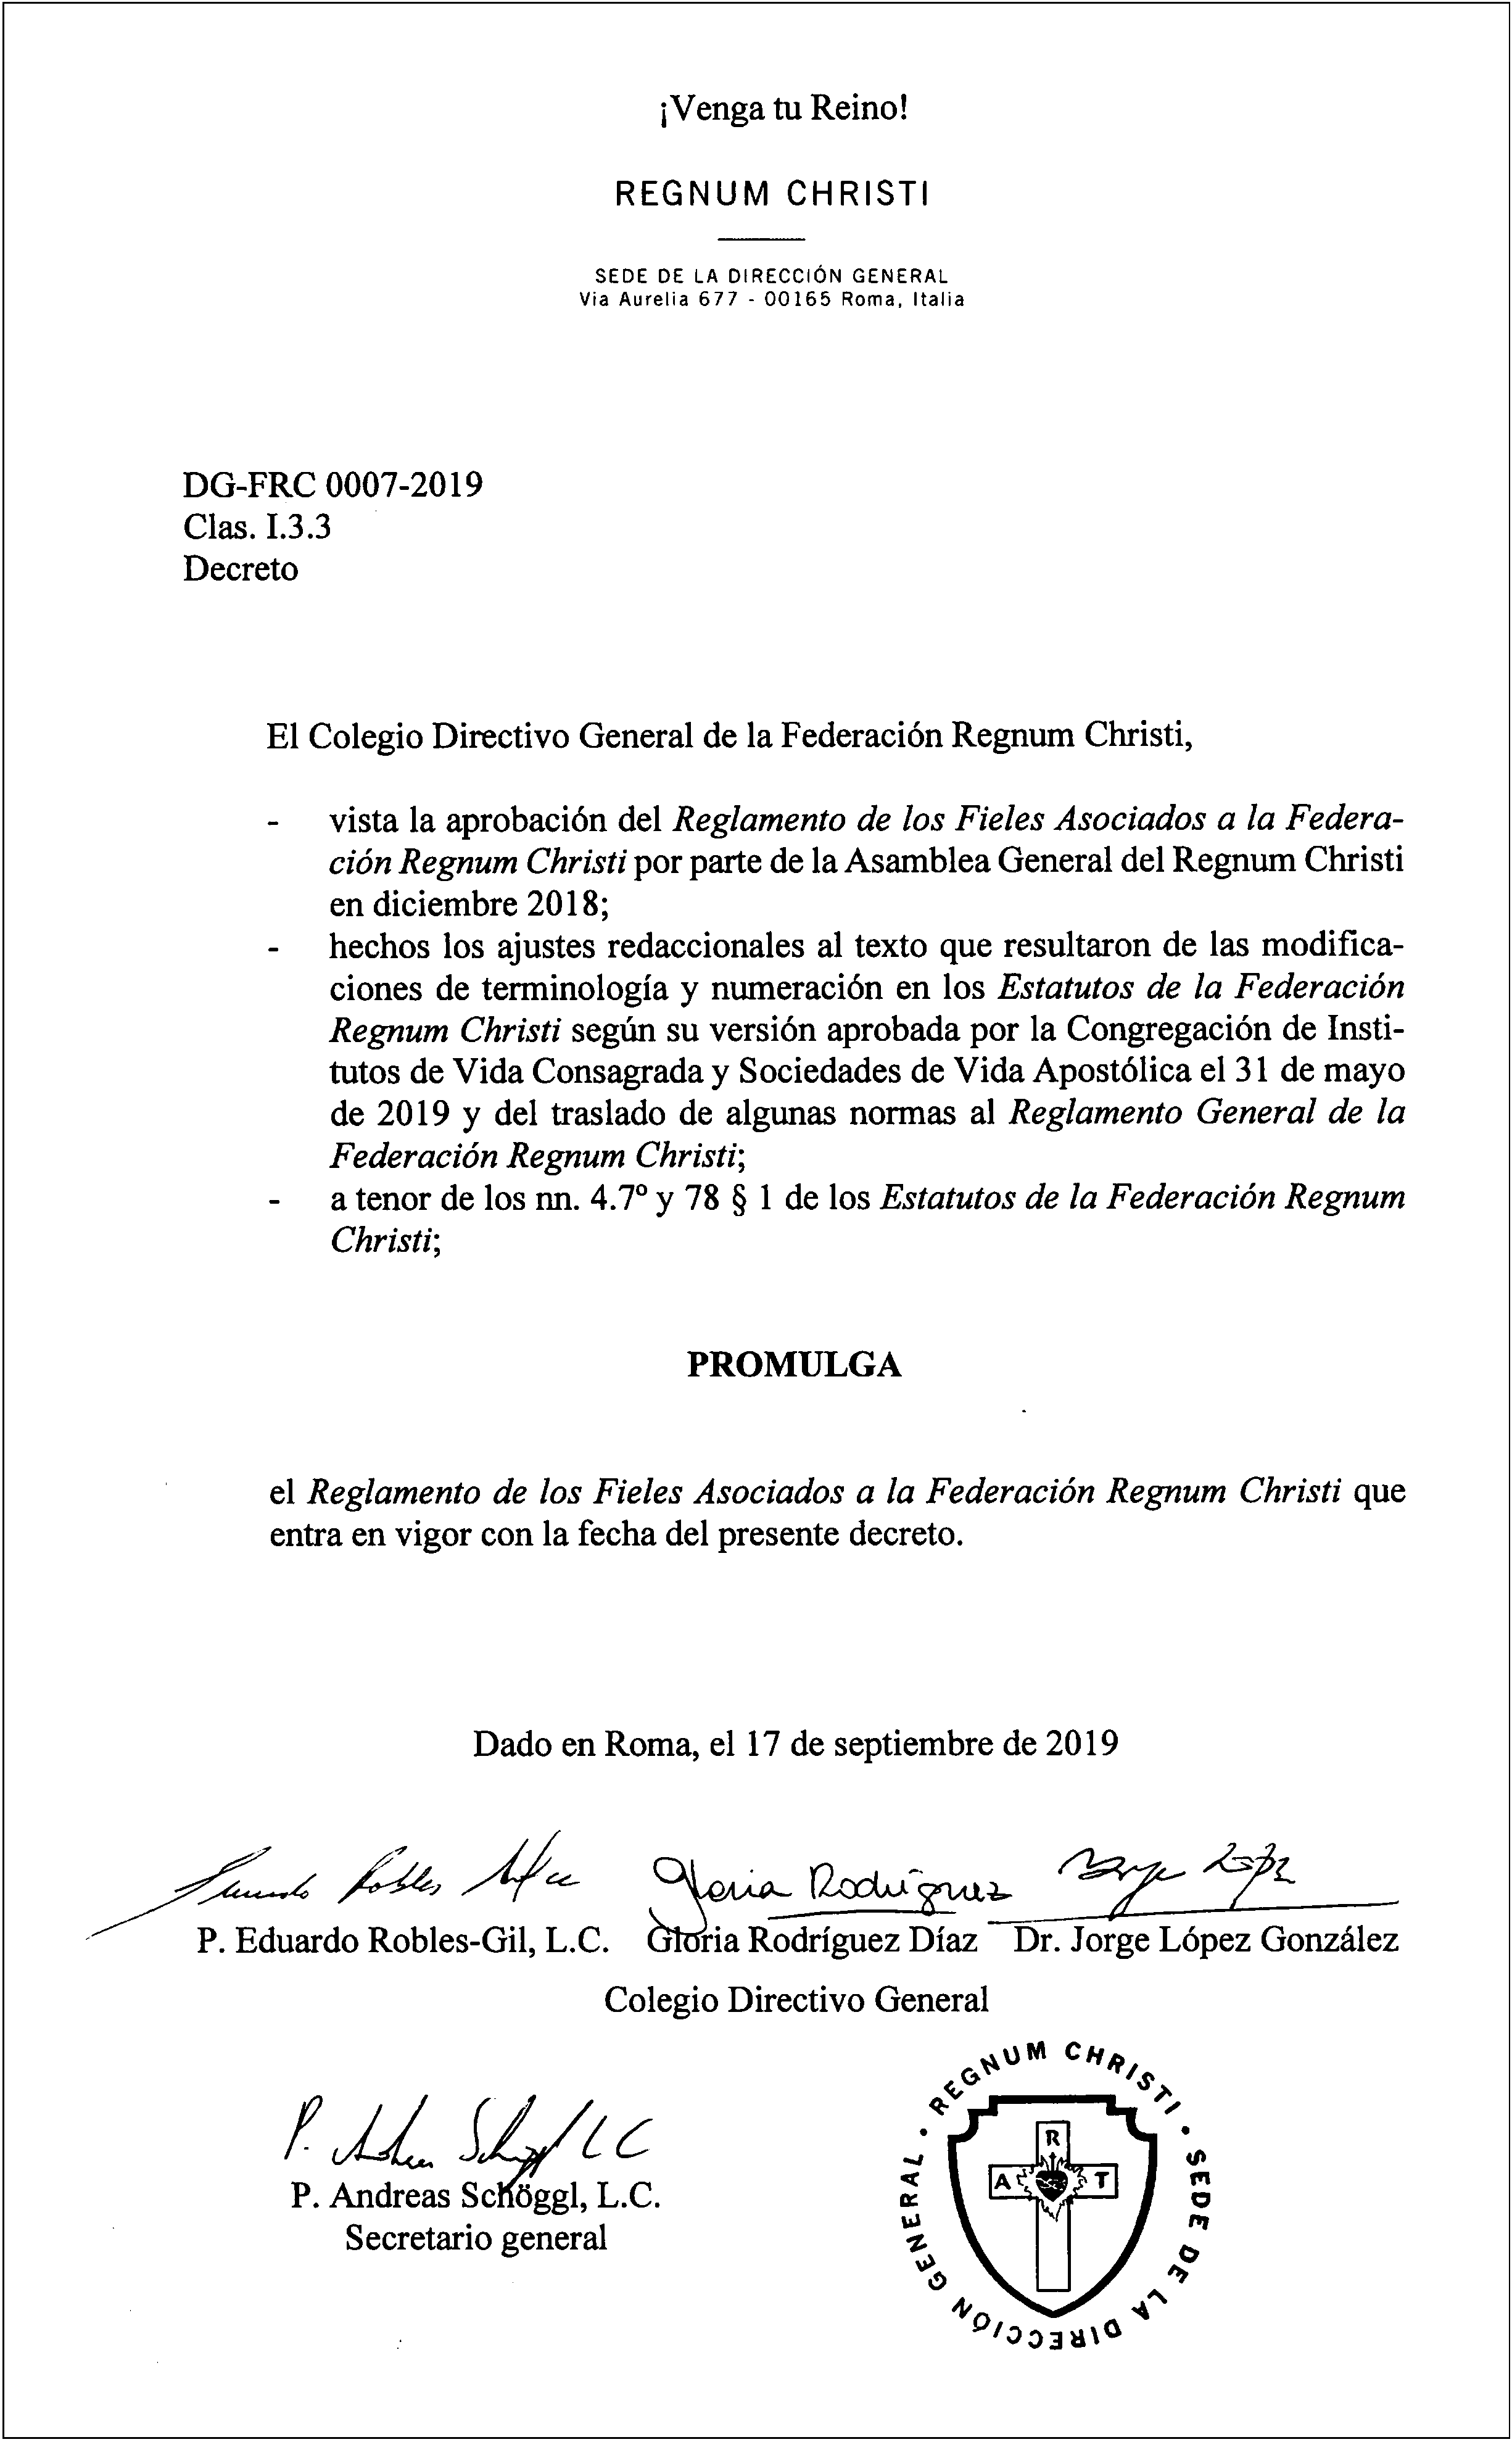
\includegraphics[height=
	\textheight]{dekret-przepisy-wiernych-stowarzyszonych} 
\end{center}
\begin{framed}
	\begin{footnotesize}
		\begin{center}
			Przyjdź Królestwo Twoje!
			
			REGNUM CHRISTI\\
			Siedziba Zarządu Generalnego\\
			Via Aurelia 677, 00165 Rzym, Włochy 
		\end{center}
		
		DG-FRC007-2019\\
		Clas. I.3.3\\
		Dekret
		
		Kolegium Generalne Federacji Regnum Christi,
		\begin{itemize}
			
			\item mając na uwadzę aprobatę Przepisów Wiernych Stowarzyszonych w Federacji Regnum Christi przez Zgromadzenie Ogólne Regnum Christi w grudniu 2018 roku; 
			
			\item uwzględniwszy poprawki w redakcji tekstu wynikające ze zmian terminologii i numeracji Statutów Federacji Regnum Christi według wersji zatwierdzonej 31 maja 2019 roku przez Kongregację ds. Instytutów Życia Konsekrowanego i Stowarzyszeń Życia Apostolskiego oraz wynikających z przeniesienia niektórych norm do Przepisów Ogólnych Federacji Regnum Christi;
			
			\item zgodnie z numerem 4.7 i 78 \S{}1 {\em Statutów Federacji Regnum Christi};
		\end{itemize}
		\begin{center}
			ZATWIERDZA 
		\end{center}
		
		{\em Przepisy Wiernych Stowarzyszonych w Federacji Regnum Christi}, które wchodzą w życie wraz z datą niniejszego dekretu.
		\begin{center}
			Podpisano w Rzymie, 17 września 2019 roku
			\begin{tabular}
				{ c c c } {\em podpis} & {\em podpis} & {\em podpis} \\
				o. Eduardo Robles-Gil, LC & Gloria Rodríguez Díaz & dr. Jorge López González \\
				\multicolumn{3}{c}{Kolegium Generalne} 
			\end{tabular}
			\begin{tabular}
				{ c c c } {\em podpis} & & \\
				o. Andreas Schöggl, LC & & {\em pieczęć} \\
				Sekretarz Generalny & & 
			\end{tabular}
		\end{center}
	\end{footnotesize}
\end{framed}

% Część pierwsza
\part{Świeccy członkowie Regnum Christi}

%Rozdział 1
\chapter{Tożsamość i styl życia świeckiego członka Regnum Christi}

\ssec{Tożsamość świeckiego członka Regnum Christi}

\lett{1} \S{}1. {\em Świeccy członkowie Regnum Christi} to wierni, którzy, bez przyjmowania zobowiązań ewangelicznych wiążących węzłem świętym, osobiście odpowiadają na Boże powołanie do przeżywania zobowiązań chrzcielnych w rzeczywistości doczesnej, według charyzmatu Regnum Christi, którego fundamentalne założenia zostały opisane w punktach 6-30 {\em Statutów Federacji Regnum Christi} oraz w niniejszych {\em Przepisach}.

\S{}2. Wierni ci przystępują do Regnum Christi poprzez indywidualne dołączenie do Federacji i przyjmowani są przez dyrektorów jej poszczególnych sekcji, zgodnie ze {\em Statutami Federacji Regnum Christi}.

\S{}3. Wnoszą oni swój świecki charakter i apostolską działalność, poprzez które uobecniają Chrystusa w świecie i dążą do ewangelicznej przemiany ludzkiej rzeczywistości, zwłaszcza życia rodzinnego, zawodowego i społecznego.\footnote{{\em Statuty Federacji Regnum Christi}, nr 5 \S{}4.}

\ssec{Elementy właściwe dla stylu życia świeckiego członka Regnum Christi}

\lett{2}\label{numerdwa}Regnum Christi proponuje chrześcijaństwo aktywne, pełne entuzjazmu i miłości; styl życia, który pomaga wypełniać zobowiązania chrzcielne i realizować misję bycia chrześcijańskim zaczynem w świecie. Świecki członek Regnum Christi rozwija ten styl życia w życiu duchowym, formacji, apostolacie, osobistym towarzyszeniu i w życiu drużyny.


\section{Artykuł 1. Życie duchowe}

\ssec{Ukierunkowanie życia duchowego}

\lett{3} Świecki członek Regnum Christi postrzega życie duchowe jako ciągły rozwój życia trynitarnego\footnote{Katechizm Kościoła Katolickiego, nr 1721} w sobie samym, prowadzący do upodabniania się do Chrystusa. Stąd przeżywa on swoje życie jako dynamiczną relację miłości z Bogiem, która karmi się sakramentami, Słowem Bożym, życiem liturgicznym, modlitwą oraz doskonaleniem cnót teologicznych i moralnych. Życie duchowe przenika i harmonizuje wszystkie obszary jego życia.

\filbreak\ssec{Świecka duchowość}

\lett{4}{} Świadomy otrzymanego na Chrzcie św. daru Bożego synostwa w Chrystusie, świecki członek Regnum Christi przeżywa swoją kapłańską, prorocką i królewską posługę w rzeczywistości doczesnej, dążąc do uobecniania Królestwa Bożego w tym świecie, by stał się on domem godnym dzieci Bożych, w którym wszystko przyczynia się do oddawania Mu chwały.

\ssec{Praktyki życia duchowego}

\lett{5} Praktyki życia duchowego proponowane świeckim członkom Regnum Christi są sposobem wzrastania w relacji miłości z Chrystusem. Świecki członek, dzięki pomocy swojego duchowego kierownika, stopniowo zagłębia się w modlitwę mentalną oraz w przeżywanie innych, zalecanych w Modlitewniku praktyk. Uprzywilejowanym sposobem osiągania wzrostu duchowego jest zalecane, coroczne uczestnictwo w ćwiczeniach duchowych albo w triduum odnowy wewnętrznej.


\section{Artykuł 2. Formacja}

\lett{6} Świecki członek Regnum Christi podejmuje ścieżkę formacji określoną w punkcie 30. {\em Statutów Federacji Regnum Christi}. Jest to ścieżka wzrostu w dojrzałości ludzkiej i chrześcijańskiej zgodnie ze stanem życia, ścieżka wspomagająca owocną współpracę apostolską, ścieżka, której celem jest oświecanie i przemiana realiów tego świata w Chrystusie. 

\filbreak\ssec{Osobista odpowiedzialność i ścieżka instytucjonalna}

\lett{7}\S{}1. Świecki członek bierze na siebie odpowiedzialność za własną formację.

\S{}2. Odpowiednie władze Federacji zobowiązane są do ustalenia planu formacyjnego, zawierającego cele, wytyczne i środki.

\S{}3. Standardowy sposób prowadzenia formacji oparty jest na kręgach studyjnych i zróżnicowanych kursach.

\ssec{Szkolenia}

\lett{8} Świeccy członkowie Regnum Christi, wyznaczeni do wypełniania obowiązków dotyczących posługi innym muszą otrzymać odpowiednie przygotowanie, towarzyszenie oraz informację zwrotną.\footnote{ang. {\em feedback}}


\section{Artykuł 3. Apostolat}

\ssec{Bycie apostołem}

\lett{9} Świeccy członkowie Regnum Christi gorliwie dążą do ustanowienia i rozpowszechnienia Królestwa Chrystusa wśród ludzi. Pozwalają, by przenikała ich miłość Chrystusa do ludzi oraz ożywiają swój zapał apostolski w intymnej relacji z Chrystusem. Pragną, by Chrystus zapanował w ich duszach oraz duszach tych wszystkich osób, które ich otaczają. Prowadzeni przez Ducha Świętego, na wzór św. Pawła, starają się mieć nadprzyrodzone spojrzenie w swoich aspiracjach, mieć wielkoduszne serce, być odważnymi w poświęceniu, wytrwałymi w trudnościach oraz praktycznymi i skutecznymi w działaniu, poszukując tym samym przemiany świata w Chrystusie. Ich mottem jest: {\em Chryste, nasz Królu: Przyjdź Królestwo Twoje!} 

Dlatego:
\begin{enumerate}
	
	%1
	\item szukają codziennego spotkania z Chrystusem na modlitwie oraz dają o Nim świadectwo w różnych okolicznościach swojego życia;
	
	%2
	\item w przeżywaniu swojego świeckiego powołania, oświeceni Słowem Bożym i nauczaniem Kościoła, w pierwszej kolejności biorą odpowiedzialność za swoje życie rodzinne i obowiązki stanu;
	
	%3
	\item starają się wychodzić na spotkanie ludziom w konkretnych sytuacjach życiowych, aby głosić im Ewangelię i zapraszać ich do współuczestnictwa w misji Chrystusa;
	
	%4
	\item przyjmują świecką odpowiedzialność za niesienie światła Ewangelii w obręb życia publicznego, kulturalnego, gospodarczego, politycznego, akademickiego i społecznego; ponadto szukają sposobu na rozbudzenie apostolskiego zaangażowania wśród różnych liderów dzisiejszego świata, aby żyli oni w większej spójności ze swoimi etycznymi i religijnymi przekonaniami;
	
	%5
	\item w miarę możliwości podejmują inicjatywy i uczestniczą w dziełach apostolskich;
	
	%6
	\item szukają sposobów uczestniczenia w życiu parafialnym i diecezjalnym, wnosząc do swojego lokalnego Kościoła charyzmat Regnum Christi;
	
	%7
	\item pragną dzielić z innymi dar Boży odkryty w Regnum Christi, dlatego umożliwiają poznanie tego daru, zapraszają do Regnum Christi i towarzyszą osobom, które okazują zainteresowanie nim lub chcą uczestniczyć w jego duchowości i misji.
\end{enumerate}

\filbreak\ssec{Wartość ECYD\footnote{{\em ECYD} to nazwa własna pochodząca od hiszpańskich słów {\em Encuentros, Convicciones y Decisiones} --- spotkania, przekonania i decyzje. Jest to nazwa międzynarodowej organizacji, w której młodzież przeżywa charyzmat Regnum Christi w sposób adekwatny do swojego wieku.}}

\lett{10} Pamiętając o tym, że młodzież ma fundamentalne znaczenie dla przyszłości Kościoła, Regnum Christi oraz całego społeczeństwa, świeccy członkowie Regnum Christi są współodpowiedzialni za otaczanie odpowiednią troską i zainteresowaniem wszystkich młodych tworzących ECYD.


\section{Artykuł 4. Towarzyszenie osobiste i wspólnotowe}

\ssec{Towarzyszenie}

\lett{11} Towarzyszenie\footnote{{\em Statuty Federacji Regnum Christi}, nr 35 \S{}1.} jest wspólną odpowiedzialnością świeckiego członka Regnum Christi, który winien o nie zabiegać i Federacji Regnum Christi, która musi starać się je zapewnić. Przejawia się ono zwłaszcza w trosce osobistej i sakramentalnej, życiu drużyny, formacji i opiece apostolskiej.

\ssec{Kierownictwo duchowe}

\lett{12} Świecki członek Regnum Christi poszukuje systematycznego kierownictwa duchowego jako, tradycyjnego w Kościele, sposobu duchowego wzrostu. Dzięki niemu uczy się rozpoznawania woli Bożej i przyjmowania jej z miłością. 

\filbreak\ssec{Dialog z osobą odpowiedzialną}

\lett{13} Świeckiemu członkowi Regnum Christi towarzyszy osoba odpowiedzialna za drużynę, która, poprzez częsty dialog z nim, wspomaga go w braterskiej i przyjacielskiej relacji na drodze rozwoju osobistego i apostolskiego.


\section{Artykuł 5. Życie drużyny}

\ssec{Drużyna}

\lett{14} \S{}1. Świeccy członkowie zazwyczaj wchodzą w skład jednej drużyny. Drużyna to naturalne środowisko, gdzie wzrasta i rozwija się ich życie w Regnum Christi.

\S{}2. Drużyna to ogół członków złączonych chrześcijańskim braterstwem, w celu wzajemnej pomocy na drodze uświęcania, formacji i pracy apostolskiej, na wzór pierwszych wspólnot chrześcijańskich.

\S{}3. Drużyny, jako wspólnoty apostołów, mogą organizować się na różne sposoby, w zależności od konkretnych możliwości regionu Federacji.

\ssec{Spotkanie z Chrystusem}

\lett{15} {\em Spotkanie z Chrystusem} znajduje się w centrum życia drużyny. W jego trakcie świeccy członkowie, jako wspólnota wiary oraz w świetle Słowa Bożego, dokonują analizy swojego życia chrześcijańskiego; rozeznają czego oczekuje od nich Pan, aby ewangelizować rzeczywistość w której żyją; zagrzewają się wzajemnie do podążania za Chrystusem oraz hartują swój zapał apostolski.

% Rozdział 2
\chapter{Przystąpienie osób świeckich do Federacji Regnum Christi}

\ssec{Duchowe znaczenie aktu przystąpienia}

\lett{16} Osoba świecka przystępując do Federacji świadomie przyjmuje chrzcielne powołania do świętości i apostolatu oraz powierza się Chrystusowi, aby to On królował w jej sercu i w społeczeństwie. W ten sposób rozpoczyna drogę asymilacji, życia duchem, wspólnotą i misją Regnum Christi opisanych w {\em Statutach Federacji Regnum Christi}, szczególnie poprzez pięć elementów właściwych życiu świeckiego członka Regnum Christi\footnote{patrz nr 2 na stronie \pageref{numerdwa}.}.

\ssec{Zobowiązania}

\lett{17} Świecki członek przystępując do Federacji zobowiązuje się do:
\begin{enumerate}
	
	%1
	\item wzrastania w przyjaźni z Chrystusem rozwijając życie łaski poprzez modlitwę i sakramenty;
	
	%2
	\item życia w duchu rad ewangelicznych ubóstwa, synowskiego posłuszeństwa oraz czystości w myślach i czynach;
	
	%3
	\item wypełniania z miłością i uczciwością obowiązków stanu jako służby Bogu i bliźnim;
	
	%4
	\item zaangażowania w formację integralną i kształtowanie swego chrześcijańskiego przywództwa;
	
	%5
	\item podejmowania inicjatyw apostolskich i uczestniczenia w nich;
	
	%6
	\item wyznawania wiernej i aktywnej miłości do Kościoła świętego, Ojca Świętego i pozostałych biskupów;
	
	%7
	\item hojnego ofiarowania swej modlitwy, talentów, czasu i środków, aby współrealizować misję Regnum Christi w służbie Kościołowi.
\end{enumerate}

\ssec{Wymagania}

\lett{18} Do Federacji może zostać przyjęty każdy katolik, który ukończył szesnasty rok życia, pragnie żyć duchem Regnum Christi, posługiwać się jego środkami uświęcania i uczestniczyć w jego działalności apostolskiej, a ponadto wykazuje się prawym postępowaniem oraz potrafi podjąć się wypełniania stosownych zobowiązań.

\ssec{Przynależność do innych instytucji w Kościele}

\lett{19} \S{}1. Ci, którzy przynależą już do innych ruchów kościelnych, a pragną być zrzeszeni w Federacji powinni, wraz z dyrektorem sekcji, rozważyć, czy ich zobowiązania zgadzają się z tymi wcześniejszymi, podjętymi w innych instytucjach.

\S{}2. Nie wyraża się zgody na dołączenie do Federacji osobom, które uprzednio podjęły rady ewangeliczne potwierdzone świętym węzłem w innej rodzinie duchowej.

\ssec{Proces przyłączenia}

\lett{20} \S{}1. Decyzja o ubieganie się o przyłączenie do Federacji musi być owocem odpowiedniego rozeznania i swobodnej odpowiedzi na wezwanie Boga.

\S{}2. Przyjęcie do Federacji leży w kompetencji dyrektora sekcji. Jest odpowiedzią na pisemny wniosek ubiegającej się o przyjęcie osoby oraz rekomendacji osoby odpowiedzialnej za drużynę, a także jednego z członków tej drużyny i następuje po odpowiednim okresie uczestnictwa w życiu Regnum Christi, które służyło wzajemnemu poznaniu się osoby zainteresowanej i dyrektora sekcji.

\S{}3. Przyjęcie ma miejsce, zwykle po triduum duchowym, poprzez formalny akt lub ceremonię, zgodnie z {\em Ceremoniałem Regnum Christi}, który musi wyrażać to, co zapisano w 16-tym i 17-tym punkcie niniejszych {\em Przepisów}. Przyjęcie zostaje odpowiednio odnotowane w aktach.

\S{}4. Świecki członek dokonuje corocznie modlitewnego odnowienia przyjętych z tytułu zrzeszenia zobowiązań, które ustanawia punkt 17-ty niniejszych {\em Przepisów}.

\S{}5. Członkowie stowarzyszonych instytucji, którzy opuszczają swoją instytucję i pragną nadal przynależeć do Regnum Christi powinni wnioskować u dyrektora sekcji o wpisanie ich w rejestr świeckich członków Regnum Christi.

\ssec{Odejście}

\lett{21} \S{}1. Każdy świecki członek, po uprzednim rozważeniu przed Bogiem swojej decyzji, ma prawo do opuszczenia Federacji po pisemnym zawiadomieniu swojego dyrektora sekcji.

\S{}2. Ze względu na całkowicie dobrowolny i bezinteresowny charakter osobistego zaangażowania, osoba opuszczająca Federację, bez względu na formę swojego odejścia, nie ma prawa zgłaszać żadnych roszczeń w związku z jakimkolwiek świadczeniem zrealizowanym na rzecz Federacji.

\ssec{Utrata przynależności {\em ipso facto}\footnote{łac. {\em na mocy samego faktu}. W prawie kanonicznym zwrot używany do określenia automatycznej natury wyłączenia ze względu na podjęty przez osobę czyn.}}

\lett{22} \S{}1. {\em Ipso facto} przestają przynależeć do Federacji Regnum Christi osoby, które podejmują rady ewangeliczne potwierdzone świętym węzłem w innej rodzinie duchowej.

\S{}2. Kto publicznie porzuca wiarę katolicką {\em ipso facto} przestaje być stowarzyszony w Federacji Regnum Christi.

\ssec{Wydalenie i jego powody}

\lett{23} \S{}1. Dyrektor sekcji, po wysłuchaniu osoby odpowiedzialnej za drużynę oraz za zgodą swojej Rady, może, z uzasadnionych przyczyn i jeśli zajdzie taka potrzeba, wydalić świeckiego członka Federacji. Przed podjęciem decyzji o wydaleniu, dyrektor sekcji, wysłuchawszy osoby odpowiedzialnej za drużynę lub grupę oraz za zgodą swojej Rady, zobowiązany jest do pisemnego upomnienia członka, ostrzegając go o możliwości wydalenia wraz z uzasadnieniem. W upomnieniu musi określić termin na ewentualną poprawę ze strony członka. Ten ostatni ma prawo do obrony przed dyrektorem sekcji. Po upływie czasu określonego w upomnieniu oraz daniu członkowi możliwości obrony, dyrektor sekcji, jeśli uzna jego wydalenie za konieczne, posiadając zgodę swojej Rady, zobowiązany jest do pisemnego powiadomienia go o wydaleniu, które winno być prowadzone w sposób sprawiedliwy, roztropny i miłosierny.

\S{}2. Wydalonemu świeckiemu członkowi Regnum Christi przysługuje prawo złożenia odwołania do Kolegium Terytorialnego.

\S{}3. Za powód do wydalenia należy uznawać publiczne i uporczywe utrzymywanie poglądów i zachowań sprzecznych z wiarą i dyscypliną Kościoła.

%Rozdział 3
\chapter{Szczególne sposoby oddania się świeckich członków Regnum Christi}


\section{Artykuł 1. Dodatkowe zobowiązania szczególne}

\lett{24} \S{}1. Niektórzy świeccy członkowie doświadczają Bożego wezwania do podjęcia szczególnych zobowiązań wobec Pana i gotowości względem Niego po to, by ożywiać życie i misję Regnum Christi. W odpowiedzi na to wezwanie podejmują się drogi modlitwy i formacji oferowanej przez Regnum Christi oraz zobowiązują się do aktywnego zaangażowania poprzez swoją modlitwę, talenty, czas i posługę.

\S{}2. Osoby przyjmujące to wezwanie stanowią wartościowe wsparcie dla sekcji oraz swoich apostolatów poprzez modlitwę, oddanie i dyspozycyjność.

\S{}3. Świecki członek Regnum Christi wraz z dyrektorem sekcji ustalają między sobą różne konkretne formy przeżywania tego oddania i dyspozycyjności w zależności od osobistych okoliczności oraz potrzeb Regnum Christi.

\S{}4. To świecki członek Regnum Christi, wspierany przez swojego kierownika duchowego, bierze na siebie odpowiedzialność godzenia podejmowanych zobowiązań z obowiązkami właściwymi dla jego stanu.

\lett{25} \S{}1. Podjęcie tych szczególnych zobowiązań wobec Regnum Christi odbywa się poprzez przyrzeczenie złożone w obecności dyrektora sekcji i kilku jej członków według zasad {\em Ceremoniału Regnum Christi}.

\S{}2. Przyrzeczenie to winno być udokumentowane i potwierdzone podpisem.

\S{}3. Przyrzeczenie to składane jest po raz pierwszy na okres jednego roku z możliwością corocznego przedłużenia. Po pięciokrotnym odnowieniu, jeśli świecki członek wyraża takie pragnienie, a dyrektor sekcji uzna to za stosowne, przyrzeczenie może zostać przyjęte {\em ad vitam}.

\ssec{Przepis przejściowy}

Ci świeccy członkowie Regnum Christi, którzy zgodnie z poprzednimi przepisami byli „członkami drugiego stopnia” co najmniej przez pięć ostatnich lat i posiadają zgodę dyrektora sekcji, będą mogli złożyć przyrzeczenie dodatkowych zobowiązań {\em ad vitam} bez potrzeby spełnienia warunków punktu 25, \S{}3 niniejszych {\em Przepisów}.

\S{}4. Dyrektorzy sekcji dbają o to, by członkowie składający to przyrzeczenie otrzymywali niezbędne towarzyszenie w wypełnianiu swej obietnicy.

\S{}5. Kompetentny organ Federacji ustala plan formacyjny, który oferuje cele, wytyczne i środki członkom, którzy złożyli to przyrzeczenie.

\ssec{Wymagania do złożenia przyrzeczenia}

\lett{26} \S{}1. Przyrzeczenie może złożyć świecki członek Federacji, który ukończył osiemnasty rok życia, postępuje w sposób prawy, stowarzyszony jest w Federacji wystarczająco długo, by dać się poznać swojemu dyrektorowi sekcji oraz z pomocą swojego kierownika duchowego przeszedł przez etap rozeznania.

\S{}2. Przyrzeczenie należy złożyć w duchu hojności i pokory wobec posługi Królestwu Bożemu oraz w mocnym pragnieniu przyczynienia się do rozwoju Regnum Christi.

\ssec{Przyjęcie przyrzeczenia}

\lett{27} Przyjęcie przyrzeczenia dodatkowych zobowiązań leży w gestii dyrektora sekcji oraz jego Rady i odbywa się na pisemny wniosek osoby zainteresowanej.

\ssec{Dyspensa}

\lett{28} \S{}1. Świecki członek Regnum Christi po dojrzałym rozeznaniu dokonanym przy wsparciu swojego kierownika duchowego może wnioskować u dyrektora sekcji o zwolnienie z przyrzeczenia.

\S{}2. Dyrektor sekcji udziela świeckiemu członkowi dyspensy w formie pisemnej, co też zostaje odnotowane w archiwum sekcji.

\filbreak


\section{Artykuł 2. Współpracownicy}

\ssec{Współpracownicy}

\lett{29} Mianem współpracowników\footnote{Historycznie używano angielskiego słowa \em{coworker}, które dalej funkcjonuje w naszym potocznym języku.} określani są ci świeccy członkowie Regnum Christi, którzy poświęcają przynajmniej jeden rok swojego życia w służbie Kościołowi poprzez pełnowymiarowy wolontariat apostolski w Regnum Christi i według obowiązujących w Federacji przepisów..

%Rozdział 4
\chapter{Struktury i posługi świeckich członków Regnum Christi}

\ssec{Drużyny}

\lett{30} \S{}1. Drużyna składa się przeważnie z osób tej samej płci, będących na tym samym etapie życia, połączonych więzią przyjaźni, pokrewieństwa lub wspólnych zainteresowań. Możliwe są również drużyny małżeństw prowadzone przez jedno małżeństwo.

\S{}2. Drużyna prowadzona jest przez osobę odpowiedzialną, wyznaczoną przez dyrektora sekcji wspieranego przez właściwą Radę i po zasięgnięciu opinii pozostałych członków drużyny. Osoba odpowiedzialna wyznaczana jest na okres od jednego do trzech lat z możliwością przedłużenia funkcji.

\S{}3. Misją osoby odpowiedzialnej za drużynę jest prowadzenie i ożywianie życia w drużynie. Jest ona przewodnikiem i formatorem, który towarzyszy każdemu członkowi w jego drodze uświęcania, w procesie formacji i w jego rozwoju jako apostoła.

\S{}4. Liczba członków w drużynie powinna sprzyjać wzajemnemu wsparciu, zawiązywaniu przyjaźni oraz aktywnemu uczestnictwu każdego z nich.

\ssec{Grupy}

\lett{31} \S{}1. W stosownych przypadkach, ze względów formacyjnych lub z powodu apostolatu, albo gdy uzasadnia to liczba drużyn, dyrektor sekcji może zorganizować drużyny w grupy.

\S{}2. Na czele każdej grupy stoi osoba odpowiedzialna, wybrana przez dyrektora sekcji po konsultacji z osobami odpowiedzialnymi za drużyny. Osoba odpowiedzialna za grupę wyznaczana jest na okres do trzech lat z możliwością przedłużenia funkcji.

\ssec{Sekcje}

\lett{32} \S{}1. Sekcja to zbiór drużyn i grup, które promują życie w modlitwie, formację integralną, rodzinnego ducha Regnum Christi, otwartość na nowych członków, wzajemne wsparcie, aktywność apostolską i gospodarność.

\S{}2. Zazwyczaj istnieje sześć sekcji: męska, kobieca, męska sekcja młodych, kobieca sekcja młodych oraz żeńska i męska sekcja ECYD.

\S{}3. Stworzenie lub usunięcie sekcji w danym regionie podlega decyzji Terytorialnego Kolegium Federacji na wniosek dyrektora lokalnego i służy wsparciu ogólnej misji, zapewnieniu lepszego towarzyszenia i sprawnej organizacji.

\ssec{Dyrektor sekcji}

\lett{33} \S{}1. Terytorialne Kolegium Federacji po konsultacji z dyrektorem lokalnym, zgodnie z punktem 52 \S{}2 {\em Statutów Federacji Regnum Christi}, powołuje dyrektora sekcji na okres trzech lat z możliwością przedłużenia funkcji. W sytuacjach wyjątkowych może być on również mianowany na okres jednego lub dwóch lat.

\S{}2. Dyrektorem sekcji winien być świecki członek Regnum Christi stowarzyszony w Federacji co najmniej trzy lata albo członek instytucji stowarzyszonej posiadający przynajmniej trzyletnie doświadczenie w pracy zespołowej w sekcjach.

\S{}3. Misja dyrektora sekcji polega na promowaniu celów sprecyzowanych w punkcie 32 \S{}1 niniejszych {\em Przepisów}.

\ssec{Rada dyrektora sekcji}

\lett{34} \S{}1. Dyrektor sekcji posiada swój organ doradczy zwany Radą, która składa się przynajmniej z czterech świeckich członków Regnum Christi.

\S{}2. Członkowie Rady mianowani są przez dyrektora lokalnego na wniosek dyrektora sekcji. Ich funkcja trwa tak długo, jak funkcja dyrektora sekcji, z możliwością jej przedłużenia.

\S{}3. Rada wspiera dyrektora sekcji przy podejmowaniu decyzji, opiniuje je i aprobuje, zgodnie z założeniami niniejszych {\em Przepisów} oraz uregulowań pochodnych.

\ssec{Kapelan sekcji}

\lett{35} \S{}1. Sekcja zazwyczaj dysponuje jednym kapelanem, który mianowany jest przez Kolegium Terytorialne.

\S{}2. Kapelan sekcji, podporządkowany autorytetowi dyrektora sekcji, propaguje oraz ożywia życie liturgiczne i sakramentalne, a także bierze udział w duchowej formacji świeckich członków Federacji.

\ssec{Formatorzy}

\lett{36} \S{}1. Formatorzy to członkowie świeccy lub członkowie instytucji stowarzyszonych, którzy biorą udział w kierowaniu sekcją i są odpowiedzialni za formację jej członków. Poświęcają się zwykle kierownictwu duchowemu, ewangelizacji, zajęciom formacyjnym, przewodzeniu drużynom i grupom oraz kierowaniu zajęciami apostolskimi.

\S{}2. W swojej codziennej pracy podlegają dyrektorowi sekcji. To on troszczy się, by formatorzy otrzymali odpowiednie przygotowanie i wsparcie w wykonywaniu powierzonych zadań.

%Rozdział 5
\chapter{Udział świeckich członków Regnum Christi w organach Federacji}

\ssec{Współudział i współodpowiedzialność świeckich członków Regnum Christi}

\lett{37} Zważając na specyfikę powołania świeckich członków do życia pełnią charyzmatu, a co za tym idzie, do współuczestniczenia w życiu i misji Regnum Christi, {\em Statuty Federacji Regnum Christi} stanowią, że świeccy członkowie powinni uczestniczyć w kierowaniu Federacją oraz w określaniu własnego sposobu przeżywania charyzmatu. Niniejsze {\em Przepisy} przedstawiają konkretną wizję ich uczestnictwa.


\section{Artykuł 1. Wybory i współuczestnictwo w Konwencji Generalnej i Terytorialnej}

\ssec{Przepis uzupełniający do punktu 68 {\em Statutów Federacji Regnum Christi}}

\lett{38} Delegaci świeckich członków Regnum Christi na Konwencję Generalną są wybierani przez i spośród delegatów świeckich członków Konwencji Terytorialnej. Liczba delegatów świeckich członków na Konwencję Generalną została określona w {\em Przepisach Konwencji Generalnej}.

\ssec{Przepis uzupełniający do punktu 59 {\em Statutów Federacji Regnum Christi}}

\lett{39} \S{}1. Aby wprowadzić w życie zalecenia punktu 59 \S{}2 {\em Statutów Federacji Regnum Christi}, delegaci świeckich członków Regnum Christi na Konwencji Generalnej tworzą Kolegium, które umożliwia przedstawienie ich poglądu na daną sprawę.

\S{}2. Delegaci świeckich członków wraz z członkami instytucji stowarzyszonych mają prawo do głosowania w kwestiach zatwierdzenia lub zmiany regulaminu Konwencji Generalnej\footnote{{\em Statuty Federacji Regnum Christi}, nr 59 \S{}3.}. Taką samą metodę stosuje się w przypadku zatwierdzenia lub zmiany innych ewentualnych aktów normatywnych ściśle traktujących o życiu świeckich członków Regnum Christi.

\ssec{Przepis uzupełniający do punktu 71 {\em Statutów Federacji Regnum Christi}}

\lett{40} Delegaci świeckich członków Regnum Christi na Konwencję Terytorialną wybierani są przez i spośród świeckich członków danego terytorium, zgodnie ze szczegółowymi przepisami przyjętymi przez Kolegium Konwencji Terytorialnej i po wcześniejszej konsultacji na Plenarium Terytorialnym.


\section{Artykuł 2. Wybór i współpraca świeckich w Kolegium Generalnym i Terytorialnym}

\ssec{Przepis uzupełniający do punktu 89 \S{}2 {\em Statutów Federacji Regnum Christi}}

\lett{41} \S{}1. W Plenarium Generalnym bierze udział sześciu świeckich członków wybranych na Konwencji Generalnej przez i spośród delegatów świeckich.

\S{}1. W przypadku rezygnacji jednego z członków, Kolegium Generalne, po wysłuchaniu pozostałych świeckich członków wspierających Plenarium Generalne, mianuje jego zastępcę.

\ssec{Przepis przejściowy}

Wybór świeckich członków w Kolegium Generalnym oraz tych uczestniczących w Plenarium Generalnym w okresie pomiędzy zatwierdzeniem {\em Statutów Federacji Regnum Christi} przez Stolicę Apostolską a zwołaniem najbliższej Konwencji Generalnej, należy do kompetencji Kolegium Generalnego.

\ssec{Przepis uzupełniający do punktu 76 \S{}3 {\em Statutów Federacji Regnum Christi}}

\lett{42} Dwaj świeccy członkowie Kolegium Generalnego są wybierani przez Kolegium Generalne spośród sześciu świeckich członków biorących udział w Plenarium Generalnym.

\ssec{Przepis uzupełniający do punktu 21 \S{}3 {\em Statutów Federacji Regnum Christi}}

\lett{43} Świeccy członkowie Kolegium Terytorialnego, po przeprowadzeniu właściwych konsultacji z dyrektorem lokalnym apostolatu, mianowani są przez Kolegium Terytorialne na okres kadencji trzech lat z możliwością jednokrotnego przedłużenia.

\ssec{Przepis uzupełniający do punktu 33 \S{}2 {\em Przepisów ogólnych Federacji Regnum Christi}}

\lett{44} Poza świeckimi członkami Kolegium Terytorialnego, na Plenarium Terytorialne powołuje się, po przeprowadzeniu właściwych konsultacji z dyrektorem lokalnym apostolatu, jednego lub kilku świeckich członków mianowanych przez to Kolegium Terytorialne.

\ssec{Konflikt interesów}

\lett{45} W przypadku konfliktu interesów wynikającego z poruszanych kwestii, świeccy członkowie Kolegium Generalnego lub Terytorialnego Regnum Christi oraz ci uczestniczący w jego zebraniach plenarnych, muszą wstrzymać swoje zaangażowanie w te kwestie, w przeciwnym przypadku zostaną oni odsunięci od funkcji przez Kolegium.

\ssec{Wydatki członków Kolegiów}

\lett{46} Federacja zobowiązuje się do pokrywania wydatków związanych z wykonywaniem pracy przez członków Kolegium Generalnego i Terytorialnego.

% Część 2
\part{Księża, diakoni i seminarzyści diecezjalni}

\ssec{Tożsamość księży, diakonów i seminarzystów diecezjalnych Regnum Christi}

\lett{47} \S{}1. Osobistej odpowiedzi na wezwanie do przeżywania swego kapłańskiego powołania według charyzmatu Regnum Christi mogą udzielić księża, diakoni i seminarzyści diecezjalni. 

\S{}2. Kapłani, diakoni i seminarzyści diecezjalni Regnum Christi przyłączają się do Federacji indywidualnie, zgodnie z zapisami niniejszych {\em Przepisów}.

\S{}3. Uczestniczą oni w duchowości, korzystają z metod uświęcania oraz duchowych i apostolskich zasobów oferowanych przez Regnum Christi.
